\chapter{Background}
\label{ch:background}

In this section, we discuss Memory Safety, \ac{WASM}, and ARM's \ac{PAC} and \ac{MTE} extensions.

\section{WebAssembly}
\label{sec:wasm}

WebAssembly~\cite{haas2017bringing}, initially designed as an alternative, high-performance compilation target to Javascript, continues to be applied in a wide variety of use cases.
\Ac{WASM} was carefully designed to allow for compilation from high-performance languages traditionally compiled to native machine code such as C, C++, or Rust, and for compilation to different native architectures.
\begin{description}
    \item[Linear memory:] \Ac{WASM} provides a linear memory that can be accessed by 32 or 64\,bit integers.
    This allows the compilers and languages to manage memory themselves, without being forced into an unnatural idiom.
    Languages may ship their own allocators, garbage collectors, and lay out data structures as is efficient.
    On the host, this linear memory can then be mapped directly to the host memory.
    \item[Structured control flow:] In \ac{WASM}, unstructured control flow is not possible.
    Indirect function calls are made through type-checked tables, with function pointers being represented as indices into them.
    Jumps are realized using a set of well-defined control flow constructs.
    This not only reduces the attack surface of programs compiled to \ac{WASM}, but also aides code generation. \todo{explain why}
    \item[Stack machine:] Since compilation targets offer different sets of registers, \ac{WASM} does not expose registers, but instead operates on a typed stack.
    The stack can be verified to be well-typed and compiled to register machines or \acp{IR} of optimizing compilers in a single pass, without making assumptions about the number of available registers.
    These can vary not only between different architectures, but also between runtimes, as they might reserve some registers for their own use (such as dedicating a register to hold some global state).
    \item[Limited datatypes:] \Ac{WASM} defines four basic data types: 32\, and 64\,bit integer and floating-point types respectively.
    Different proposals add \mbox{vector-}, \mbox{garbage-collected-}, and reference types, which cover other use cases.
    There is no distinction between pointer- and integer types, however.
    While this drops information, such as pointer provenance, from the original program, and prevents optimizations, this is not considered a problem.
    \Ac{WASM} is intended to be generated by an optimizing compiler, which should perform optimizations that require pointer provenance.
\end{description}

Since its inception, WebAssembly has expanded its utility beyond the initial design goal to various other domains, such as Function as a Service (FaaS) workloads, as an alternative to containers within Docker, as an isolation mechanism to allow untrusted code to be run within native applications, among other uses.

\subsection{WebAssembly Sandbox}
\label{subsec:webassembly-sandbox}
When accessing memory, the \ac{WASM} runtime must ensure the access is within the bounds of the accessible linear memory.
Then, the memory access is performed relative to the memory's base address.
In current runtimes, this is usually achieved using two major approaches.
\begin{enumerate}
    \item Explicit bounds checks: An explicit bounds check is inserted before each memory access, comparing the index with the bound of the current memory.
    \item Guard pages: When running 32\,bit \ac{WASM} on 64\,bit hosts, the runtime can leverage the fact that virtual memory is abundant.
    For each linear memory, $2^{32}$\,bytes, or 4\,GiB of virtual memory are allocated, with the memory beyond the guard being marked as inaccessible.
    The MMU will catch accesses into these pages and the operating system will deliver a segmentation fault to the runtime, which in turn will deliver a trap to the \ac{WASM} program.
\end{enumerate}


While the design of WebAssembly is designed to prevent malicious or erronous programs from compromising the host, buggy programs are still vulnerable to classical memory safety errors discussed earlier, such as buffer overflows.

\section{Memory Safety in the context of WebAssembly}
\label{sec:memory-safety}

Programs written in languages like C or C++ are prone to memory safety bugs such as memory accesses to out-of-bounds or dangling pointers, which are the fundamental attack primitives enabling a whole class of attacks on a vulnerable or buggy program~\cite{szekeres2013sok}.
Approaches to tackle these issues exist in several forms.
Programs may be written in managed languages that prevent these attacks by either not providing raw pointer accesses, such as Java, Python, JavaScript, or others.
In these languages, access to memory is either performed through bounds-checked arrays or through managed objects, such as classes.
The runtime cleans up dangling objects through a garbage collector, they cannot be manually deallocated.
This results in all references pointing to valid objects and all memory accesses being bounds-checked.
Other languages, such as Rust, take a different approach.
In safe Rust, the type system forbids many cases of invalid programs, e.g., dangling references or raw pointer accesses.
An escape hatch in the form of unsafe exists, which allows dropping down to the level of C, being able to directly manipulate raw bytes.
Both these approaches represent a fundamental tradeoff.
Managed memory, either in the form of reference-counting, or through a garbage collector incurs an overhead that may or may not be tolerated in some environments.

Studies show that in large software projects, memory safety bugs make up between 70 and 75\% of all issues~\cite{chromium_memory_safety,microsoft_memory_safety,android_memory_safety}.

\citeauthor*{lehmann2020everything} show that while some attack surfaces, such as jumping to arbitrary addresses or injecting shellcode, are mitigated by the design of WebAssembly, buffer overflows or dangling pointer accesses are still possible~\cite{lehmann2020everything}.
Since WebAssembly does not provide separate read-only memory regions, this opens up other surfaces, allowing attackers to potentially overwrite static data, since compilers place these in readable and writeable memory.

\subsection{Software-Based Mitigations}
\label{subsec:software-based-mitigations}

To mitigate memory safety bugs in languages that do not provide safety guarantees at the language level, software-based approaches to detect these errors exist.
Checks can be inserted automatically at the compiler level, which is an approach chosen by \ac{ASAN}~\cite{serebryany2012addresssanitizer}.
\ac{ASAN}incurs a large overhead, on average 73\%, which is too large to be deployed in production and is usually only tolerated while testing or fuzzing software.
A sampling based version of \ac{ASAN}, GWP-Asan, is deployed in production in several large projects, which results in a low overhead, but no full protection for a single process~\cite{serebryany2023gwp}.
On a large scale, however, this approach allows for discovery of real-world bugs that may not be triggered by testing or fuzzing workloads.

\section{Memory Safety Hardware Extensions}
\label{sec:memory-safety-hardware-extensions}

As an alternative to flexible, but slow software solutions to detect and prevent memory safety issues, CPU designers have come up with several hardware extensions designed as a building block.
These provide important primitives, that can be used to provide full or partial memory safety to programs, while also having a small enough footprint to be able to ship these solutions in production.

\begin{figure}[t]
    \centering
    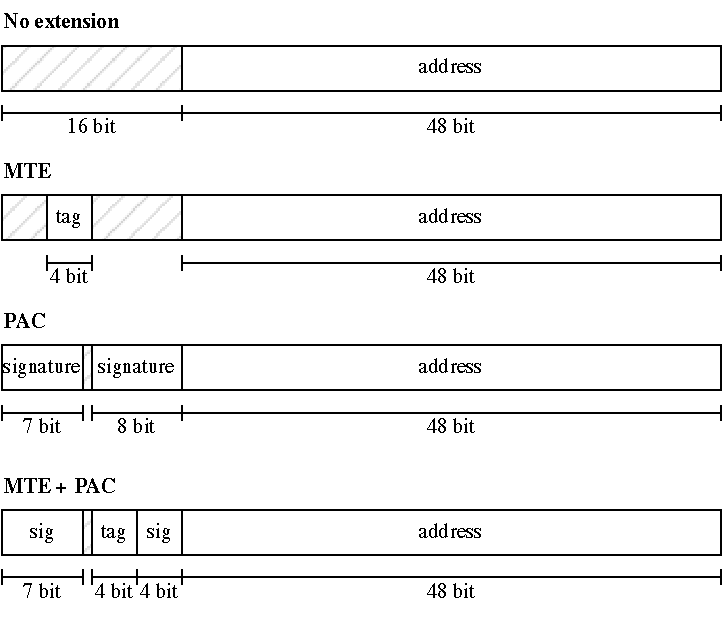
\includegraphics[scale=1]{figures/build/pointer-aarch64}
    \caption{Pointer layout on aarch64 with and without MTE and PAC enabled}
    \label{fig:aarch64-pointer}
\end{figure}

In \cref{fig:aarch64-pointer}, the layout of pointer bits used for address translation in aarch64, the 64\,bit variant of the ArmV8 instruction set, is shown.
Only 48 out of the available 64\,bits are used to address memory, while the remaining bits are set to either 0 or 1 to differentiate between kernel and userspace addresses, but unused for further address translation.
 Hardware extensions such as MTE (\cref{subsec:mte}) and PAC (\cref{subsec:pac}) utilize those unused bits to store metadata.

\subsection{Memory Tagging Extension (MTE)}
\label{subsec:mte}

ARMs Memory Tagging Extension, available from armv8.5, provides a building block to prevent both spatial and temporal memory safety violations~\cite{ARM2019MTE}.
MTE implements a lock-and-key mechanism where memory regions can be tagged with one of 16 distinct tags, and memory accessed are only allowed using pointers with the corresponding keys.

The locking mechanism is implemented by storing a 4\,bit tag in bits 56-59.
Accordingly, a tag is assigned to every 16\,bytes of tagged memory.
When accessing memory with a mismatched tag, depending on the selected configuration, either a synchronous or asynchronous exception is thrown by the hardware.
Synchronous exceptions trigger a signal to the application immediately, and the memory access does not succeed.
Asynchronous exceptions are not triggered immediately and the memory access succeeds.
On the next entry to the kernel, the signal is delivered to the application.

\subsection{Pointer Authentication (PAC)}
\label{subsec:pac}

Pointer Authentication (PAC)~\cite{Qualcomm2017PointerAuth} introduces primitives to prevent attackers from modifying pointers stored in memory.
The extension provides three instructions that can be used to sign pointers, and sign or strip the signature from pointers.
The signature is stored in the upper 16 bits of pointers, with the exact layout dependent on the Operating System, hardware, and other factors, such as if MTE is enabled.
Signed pointers are invalid and cannot be used to address memory.
They are created using the \texttt{pac*} instructions.
Before being used, the signature needs to be removed.
This happens either with the \texttt{aut*} instructions, which remove the signature if it is valid, or produce a pointer that will trap when used, if the signature does not match the address.
To remove the signature regardless if it is valid, the extension provides \texttt{strip} instructions.

\paragraph{} Both MTE and PAC can be combined at the cost of bits available for the PAC signature.
The exact layout of the PAC signature varies depending on the system.
